\section{Messdaten}
\label{sec:Messdaten}

Für die Durchführung der Experimente wurden zwei Zylinder mit gleicher Höhe $h=50~\si{\milli\metre}$, aber unterschiedlicher Grundfläche, als Spulenkörper verwendet. Die Grundfläche der einen Spule ($SP_K$) entspricht einem Kreis mit Radius $r=10~\si{\milli\metre}$, die der zweiten Spule einem Quadrat ($SP_Q$) mit Seitenlänge $s=20~\si{\milli\metre}$. Die Experimente werden in \autoref{sec:Auswertung} näher ausgeführt. Zur beispielhaften Darstellung der Rohdaten ist hier der, absichtlich herbeigeführte, Abriss des Drahtes während einer Wickeloperation dargestellt.

% \begin{figure}[H]
%     \centering
%     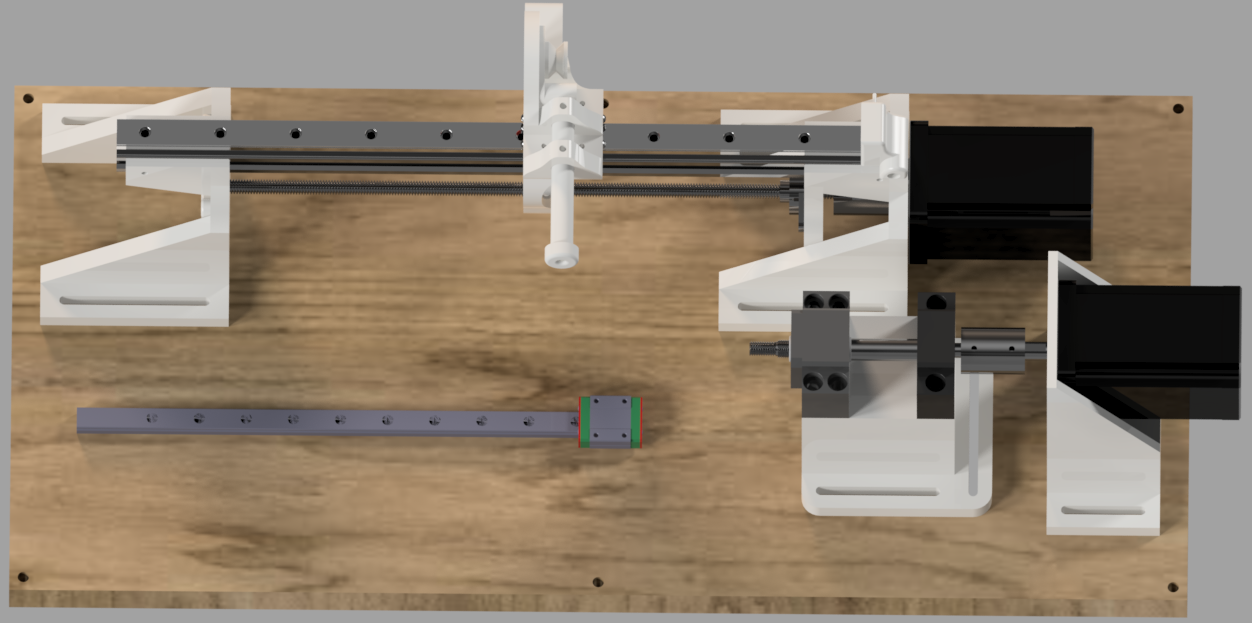
\includegraphics[width=0.25\textwidth]{./winder_render.png}
%     \caption{a nice plot}
%     \label{fig:winder_render}
% % \end{figure}
% \begin{wrapfigure}{l}{0.35\textwidth}
%     \centering
%     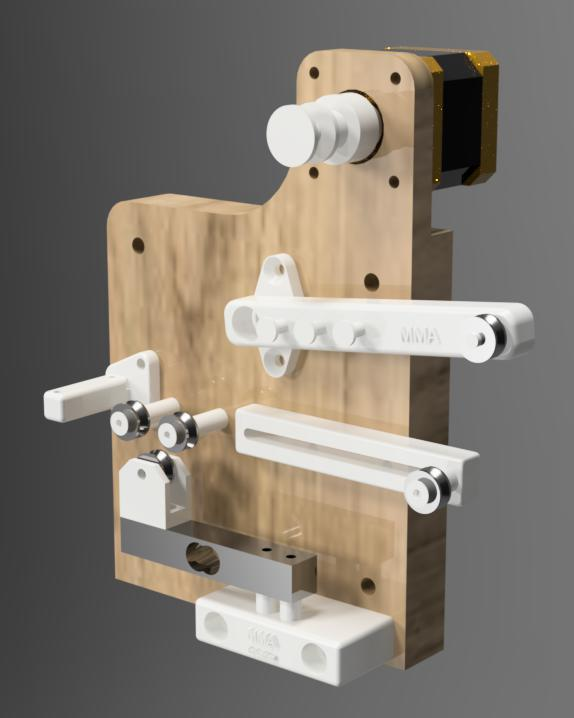
\includegraphics[width=0.35\textwidth]{./spannplatte_render.jpg}
% \end{wrapfigure}